\section{Problem Definition}

This section defines the graph fusion schedule and formulates the problem.

\textbf{Computation Graph.}
Computation graphs are a common way to represent prgrams in deep learning frameworks.
A transformer model is defined by a computation graph $G=(V, E)$, where $V$ is the set of vertices. Each vertex can represent an operator such as gemm and convolution
opertation in the computation graph. And $E$ is the set of edges which can describe the relationship between a pair of vertices. Each edge $(u, v)$ is a tensor that can 
store the output of operator $u$ and the input of operator $v$. 
Figure \ref{fig:fig1} shows the computation graph of the encoder in transformer model. \\

\begin{figure}[htbp]
    \centering
    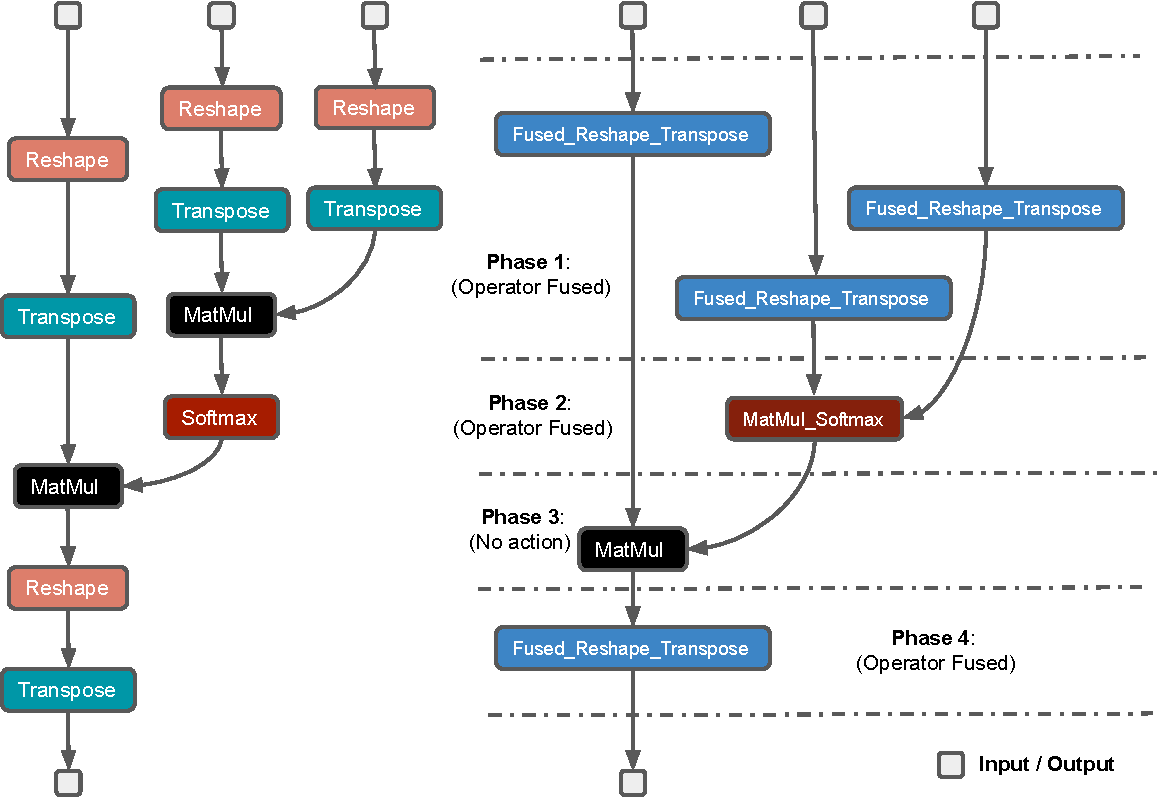
\includegraphics[width=.98\linewidth]{fig1}
    \caption{xxx}
    \label{fig:fig1}
\end{figure}


\textbf{Operator Pattern.}
Operator fusion combines multiple operators which are in adjacent positions into a single kernel rather than storing the intermediate results in the 
global memory. This optimization can greatly improve speed-up, particularly in throughput oriented architectures such as GPUs. In order to combine operators
efficiently, we should define the pattern of each operator in the computation graph. Specificaly, we set the transfomer model as our optimization goal. In TVM, 
it recognize four categories of graph opertators: (1) \textit{injective} (one-to-one map), (2) \textit{reduction}, (3) \textit{complex-out-fusable} (can fuse
element-wise map to output), and (4) \textit{opaque} (can not be fused by any operator). And it provides generic rules to fuse these operators. From
the background section, we know that transpose of matrix, batch matrix multiplication, layer normalization, softmax, and dense layer occur frequently in the 
transformer computation graph. In the meantime, the default configuration of the operators in TVM are as follows. Softmax is tagged as opaque pattern.
Batch matrix multiplication and dense are tagged as complex-out-fusable pattern. Layer normalization can be decomposed to be a set of add/subtract/multiple operators
which are all tagged as element-wise pattern. The fusion strategy is discussed below. \\


% injective, 
% reduction, 
% complex-out, 
% opaque
% # Elementwise operator
% ELEMWISE = 0
% # Broadcast operator
% BROADCAST = 1
% # Injective mapping
% INJECTIVE = 2
% # Communication
% COMM_REDUCE = 3
% # Complex op, can still fuse ewise into it
% OUT_ELEMWISE_FUSABLE = 4
% # Represents tuple node
% TUPLE = 7
% # Not fusable opaque op
% OPAQUE = 8


\textbf{Fusion Strategy and Schedule.} 
We define a schedule $S$ of a computation graph $G$. The scheduling can be defined as:
\begin{equation}
    S = \left\{(V_1, F_1), (V_2, F_2), ..., (V_k, F_k)\right\},
\end{equation}
where $V_k$ represents a group of computation operators in the \textit{i}-th phase and $F_k$ is a pair to descirbe the fusion relationship between node $v_i$
and $v_j$. For instance, the schedule for Figure xxx can be sketched by xxx.
Computation graph can be executed under the schedule $S$ from the first phase $(V_1, F_1)$ to the last phase $(V_k, F_k)$ consecutively.\\

% some common schedules for tensor program generation:split, reorder, fuse, compute_at, tile, parallel, vectorize, unroll, bind, compute_inline


\textbf{Problem Formulation.}
In order to reduce the runtime of the whole compuation graph on GPU, we set $Cost$ as a cost function on a computation graph $G$ and 
fusion schedule $S$. Our goal is to find a schedule $S^*$ to minimize the cost function for a computation graph $G$.

\begin{equation}
    {S^*} = \mathop{argmin}\limits_{S} \ Cost(G, S)
\end{equation}
The goal of the optimization is to make computation graph have low latency on the NVIDIA GPU. Therefore, we use the latency of executing executing computation 
graph $G$ according to schedule $S$ as the cost function. \\




\label{sec:form}
